%reset references counter
\setcounter{NAT@ctr}{-1}
\cleartorightpage
\chapter*{}\label{chapter:phages}
\phantomsection\addcontentsline{toc}{section}{Galaxy and Apollo as a biologist-friendly interface for high-quality cooperative phage genome annotation}

\begin{figure}[t!]
\centering
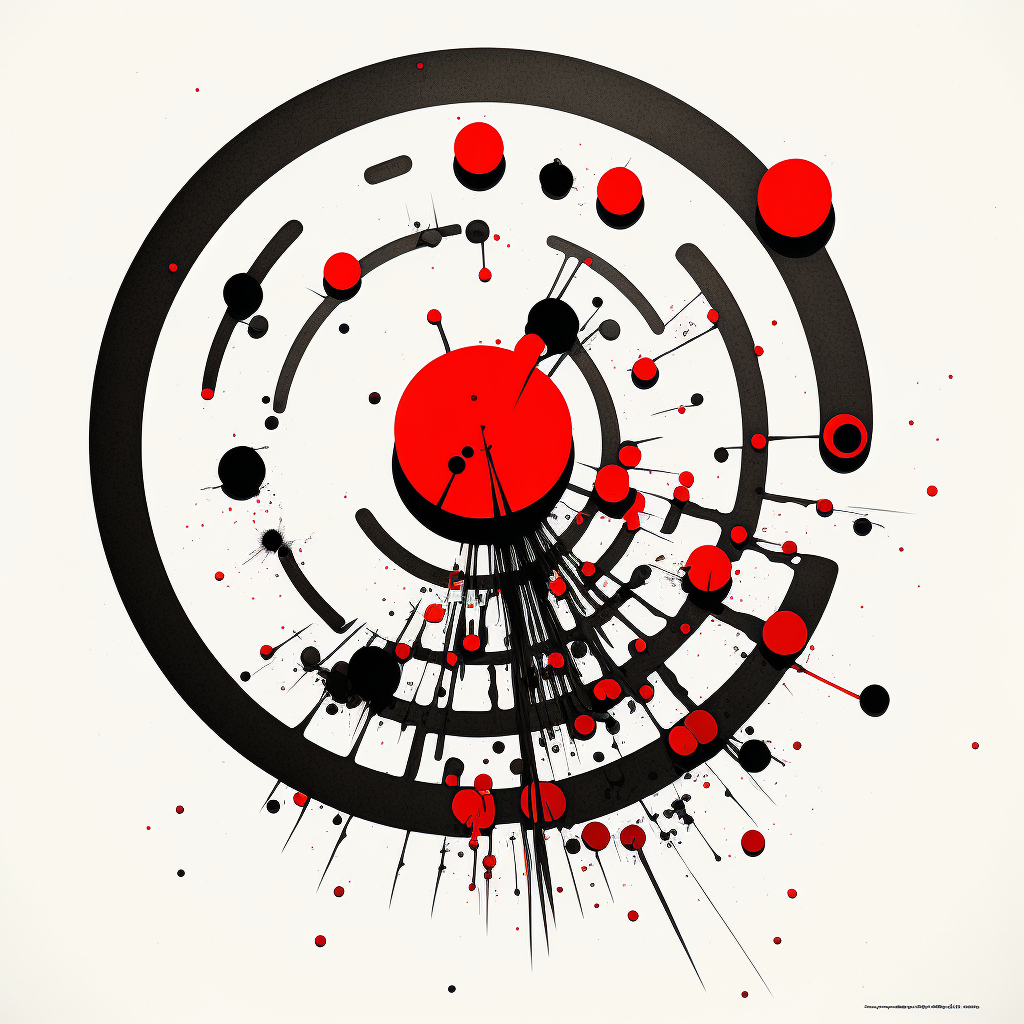
\includegraphics[height=10em]{chapters/annotation/phages.png}
\end{figure}
\vspace{-4cm}

\begin{changemargin}{0cm}{2cm}
\articletitle{Galaxy and Apollo as a biologist-friendly interface for high-quality cooperative phage genome annotation}
\end{changemargin}

Helena Rasche\textsuperscript{\ref{phage-affil:1},\ref{phage-affil:2}§},
Jolene Ramsey\textsuperscript{\ref{phage-affil:1},\ref{phage-affil:2}§},
Cory Maughmer\textsuperscript{\ref{phage-affil:1},\ref{phage-affil:2}},
Anthony Criscione\textsuperscript{\ref{phage-affil:1},\ref{phage-affil:2}},
Eleni Mijalis\textsuperscript{\ref{phage-affil:1},\ref{phage-affil:2}},
Mei Liu\textsuperscript{\ref{phage-affil:1},\ref{phage-affil:2}},
James C. Hu\textsuperscript{\ref{phage-affil:1},\ref{phage-affil:2}\dag},
Ry Young\textsuperscript{\ref{phage-affil:1},\ref{phage-affil:2}},
Jason J. Gill\textsuperscript{\ref{phage-affil:1},\ref{phage-affil:3}},

\textbf{Published in:} \emph{PLOS Computational Biology}, November 2, 2020 \\

\doi{10.1371/journal.pcbi.1008214}

\small

\begin{enumerate}
\itemsep-0.5em
\item Center for Phage Technology, Texas A\&M University, College Station, Texas, United States of America.\label{phage-affil:1}
\item Department of Biochemistry and Biophysics, Texas A\&M University, College Station, Texas, United States of America.\label{phage-affil:2}
\item Department of Animal Science, Texas A\&M University, College Station, Texas, United States of
America.\label{phage-affil:3}
\end{enumerate}

§ These authors contributed equally to this work.
\dag Deceased


\section*{Introduction}

Apollo's design is based on the premise that the best genomic
descriptions (`annotations') can be produced by starting with
automatically-generated sequence features and then providing expert
researchers with interactive editing tools to examine these multiple
sources of evidence and collaboratively refine the genomic annotations.
The first version of Apollo was a standalone desktop application
{[}1{]}. As software technologies advanced, each new generation of
Apollo took advantage of these to improve the user experience. The most
fundamental change occurred circa 2010 when Apollo transitioned to
running inside a web browser {[}2{]}. Once Apollo became a web-based
application that permits real-time collaboration, the user base grew to
include research and teaching environments studying a wide variety of
species. Our most recent version of Apollo {[}3{]} offers a broad range
of researchers an accessible way to improve the biological precision of
their genomic feature descriptions.

Organizations that use Apollo include Echinobase {[}4{]}, Hymenoptera
Genome Database {[}5{]}, i5k Workspace {[}6{]}, PhytoPath {[}7{]},
TreeGenes {[}8{]}, Vectorbase {[}9{]} and XenBase {[}10{]}. To date, the
i5K Workspace has supported publication of seven insect genomes that
were manually curated with Apollo {[}11--17{]}. Other projects that have
used Apollo include genomes of additional insects {[}18--20{]}, human
parasites {[}21--23{]}, birds {[}24,25{]}, the sea lamprey {[}26{]},
plants {[}27--29{]}, fungi {[}30--35{]} and a plant pathogenic nematode
{[}36{]}. Projects such as the re-annotation of the whipworm genome by
hundreds of high school students in the UK, supported by the Institute
for Research in Schools (IRIS) {[}37{]}, and the curation of 33,044 gene
loci in the kiwifruit genome by 93 annotators, are evidence of Apollo's
robust support for large dispersed projects.

The ease of setting up Apollo makes it appealing to small projects as
well as large. For example, one small group used Apollo to annotate 14
genes of a fungal mitochondrial genome {[}32{]}. Other reported Apollo
use cases include annotating gene loci that pose challenges in automated
gene prediction, such as the MHC-B region in the genome of the Mikado
pheasant {[}25{]} and the effector complement of the flax rust pathogen
Melampsora lini {[}33{]}. Through the process of gene model curation,
the use of Apollo can reveal species-specific genome characteristics
that can be used to improve automated gene prediction. For example,
curation of some gene models of the yellow potato cyst nematode,
\emph{Globodera rostochiensis}, using RNAseq alignments as evidence,
revealed a high frequency of non-canonical splice sites. Subsequent use
of these manually curated genes as a training set markedly improved the
automated gene predictions {[}36{]}.

Thanks to its ability to simplify and accelerate annotation efforts for
both large and small projects, Apollo's user base continues to grow.
Since 2015, Apollo has had an annual growth rate of roughly 70\% for
returning users, peaking at over 2,700 unique users one day in late
2017, with a current average of around 1,000 unique users per month.

Apollo's integrated graphical environment allows users to browse and
modify the location(s) and other information for a variety of feature
types and streamlines common editing tasks by providing built-in
calculations for features such as predicted proteins, splice sites, and
gene set membership. An overview of the interface is shown in
\protect\hyperlink{pcbi.1006790.g001}{Fig 1}.

\begin{figure}
\hypertarget{pcbi.1006790.g001}{%
\centering
\includegraphics{info:doi/10.1371/journal.pcbi.1006790.g001}
\caption{The Apollo Genome Editor has two main panels: A Genomic Editing
Workspace and a closeable Information and Administration Panel which
contains a range of configurable tabs.\\
Within the \textbf{Genomic Editing Workspace}, the \textbf{Navigation
Area} offers several ways to move to a region of interest. A user may:
move upstream or downstream in fixed units; zoom in or out; or enter the
coordinates or feature identifier to center on an exact genomic
location. The \textbf{Evidence Area} contains data imported from local
or remote files. In the \textbf{Editing Area} users can create
annotations by dragging up evidence to create editable features of
various types: coding and non-coding transcripts, pseudogenes, repeat
regions, transposons, variant calls, transcription and translation start
sites, and others. In the above example, the evidence area shows that
there are reads spanning across exons that belong to two separate,
previously known transcripts---NM\_001192578.2 and XM\_002689480.4. In
the editing area, we add these known transcripts as annotations and then
merge the two transcripts to create a single transcript. This newly
created annotation then goes through additional refinements, to ensure
that the transcript is a faithful representation of the evidence
observed.}\label{pcbi.1006790.g001}
}
\end{figure}

To briefly describe the basic capabilities, Apollo's Genomic Editing
Workspace (bottom left of \protect\hyperlink{pcbi.1006790.g001}{Fig 1})
displays tracks of information gathered from upstream pipelines and
individual users' analyses. These provide the evidence (predictions and
alignment) for refining genomic annotations. Any combination of features
can be dragged from the evidence area into the editable area, where
researchers carry out their edits without affecting the features from
the evidence area. When evidence features are dropped into the editable
track, they are assigned a default feature type of ``protein coding
transcript'' and the longest open reading frame is automatically
calculated, as well as its gene membership based on overlap with the CDS
in the same reading frame as existing transcripts. Exon boundaries can
be set either by dragging them upstream or downstream, or by using a
menu option to set them to the nearest upstream or downstream splice
junction (these are automatically calculated based on the configured
donor and acceptor dinucleotides).

Apollo provides several ways to customize the display. From the track
tab, in the information and administration panel on the right, users can
select the specific evidence tracks they want to view, categorize and
filter tracks, and change the track order. The annotation tab lists
every annotation across the genome, and can be searched by scaffold,
identifier, researcher, or biological type. Information such as the gene
symbol, description, cross-references, Gene Ontology functional class,
links to publications, or general comments on each annotation may also
be added from this tab. The reference sequence tab provides a sortable
and searchable list of every scaffold, including the length, name, and
number of annotations on each, for navigation across the genome.

\section*{Design and implementation}

Apollo's design has always been driven by its users; their engagement in
the development process has been a critical factor in Apollo's success.
Over time the demographic of Apollo users has changed, with concomitant
changes to Apollo's requirements. Notably, as sequencing costs have
fallen, there are now a burgeoning number of projects targeting specific
organisms, clades, or populations that frequently lack the funds or
expertise to create their own software tools from scratch and are
therefore reliant on available open source applications. Because members
of these projects may be geographically distributed, they need tools
that enable \textbf{real-time collaborative editing}. Additionally,
annotating the effects different \textbf{variants} have on known genes
has become a high priority research focus. And finally, particularly for
collaborative projects, tracking the complete \textbf{annotation
history} is crucial, not only for undo/redo operations but also to
review the changes that have been made over time by different
individuals.

\subsection*{Real-time collaborative editing}

Apollo was designed with a standard client-server architecture
(\protect\hyperlink{pcbi.1006790.g002}{Fig 2}) that can be run within a
servlet container (e.g., Tomcat) and works with most relational database
engines (e.g., PostgreSQL). The architecture provides a uniform
authorization layer for external applications using its web services.
For example, the i5K's project management software leverages Apollo web
services to register new users and set appropriate user and group
membership. The newly added users then have the necessary credentials to
perform manual edits or utilize the same web services, allowing them to
perform operations such as uploading bulk annotations.

\begin{figure}
\hypertarget{pcbi.1006790.g002}{%
\centering
\includegraphics{info:doi/10.1371/journal.pcbi.1006790.g002}
\caption{Apollo's client-server architecture.\\
The server is built over the Grails framework using a relational
database backend (RDBMS), for example PostgreSQL, MySQL or H2. Genomic
evidence is provided by pointing to existing JBrowse directories that
contain processed biological data. The Apollo Genome Editor and Web
Services clients communicate with the server via REST and
WebSockets.}\label{pcbi.1006790.g002}
}
\end{figure}

Apollo's client interface is built as a JBrowse {[}38{]} plugin, a
popular genome browser written in JavaScript. It provides the ability to
import and export standard genomic data formats, flexible display of
multiple types of genomic features, and fast scrolling and zooming. The
primary editing client is a single-page application that embeds JBrowse.
The server is built using Grails {[}39{]}, an open source framework for
developing web applications using Groovy {[}40{]} and other JVM
languages. The Grails framework enables us to leverage well established
technologies such as Spring
(\href{https://spring.io/}{https://spring.io}) for event control, the
Grails Object Relational Mapper (GORM), Hibernate
(\href{http://hibernate.org/}{http://hibernate.org}) for efficiently
mapping data objects to a backend persistent store, Ivy and Maven for
build and plugin dependencies, and Grails plugins for security and
navigation. Communication between the client and the server is provided
through a REST API secured by the Apache Shiro library
(\url{https://shiro.apache.org/}). To support integration into larger
workflows, the web services that support user-interface functionality
are fully exposed.

Concurrent editing by multiple users is implemented via WebSockets.
WebSockets are well-supported in most recent web browsers and are an
ideal technology to support push operations to all connected clients
efficiently in real-time. Once a user's client connects to the server,
WebSockets keep the line open for subsequent communication, including
any structural and functional editing operations. This makes every
annotation update in one client instantaneously visible in every other
client. Apollo uses the STOMP (Streaming Text Oriented Messaging
Protocol) protocol which uses a publish and subscribe communication
style, minimizing communication overhead. WebSockets provide a robust
and performant solution for pushing updates to multiple web clients that
can fall back to a more traditional long-polling approach when client
support is lacking as in older browsers.

\subsection*{Variants}

In addition to allowing genomic features to be viewed and edited, Apollo
provides the ability to annotate alterations in the underlying genomic
sequence and visualize their impact
(\protect\hyperlink{pcbi.1006790.g003}{Fig 3}). These may be assembly
error \emph{corrections}, to correct errors introduced in the sequencing
and/or assembly process (a common issue when dealing with low-coverage
genome sequences). Or these may be naturally occurring \emph{variants},
genomic differences found among different members of a population. The
effect of the annotated variants are reflected within the annotated
genomic features they intersect with.

\begin{figure}
\hypertarget{pcbi.1006790.g003}{%
\centering
\includegraphics{info:doi/10.1371/journal.pcbi.1006790.g003}
\caption{Example of variant annotation in Apollo.\\
A) AMPD2-223, an isoform of gene AMPD2 as seen from the Evidence Area
(truncated for space). From AMPD2-223, an isoform is dragged into the
Editing Area. B) The deletion variant rs1085307727, from the `Homo
sapiens Clinically associated variants' track, overlaps with
AMPD2-223-00001. Creating a corresponding deletion in the Editing Area
of the Sequence Track allows visualization of the effect of the variant
on transcript AMPD2-223-00001. Here, the transcription start site has
moved further downstream, as indicated by the red dashed line. In this
case, the altered form of the transcript recapitulates other alternate
isoforms for this gene (AMDP2-218 and AMPD2-222), which are circled and
starred for clarity.}\label{pcbi.1006790.g003}
}
\end{figure}

\subsection*{Annotation history}

As researchers progressively refine the sequence features on a genomic
region, information is automatically recorded for every change they
make: what change was made; the time and date of the change; and the
username (or email) of the editor. This edit history was a key design
requirement, ensuring that all changes made are captured in a
revertible, visual history of structural edits
(\protect\hyperlink{pcbi.1006790.g004}{Fig 4}), which lets users
graphically navigate through the different versions and roll back if
necessary.

\begin{figure}
\hypertarget{pcbi.1006790.g004}{%
\centering
\includegraphics{info:doi/10.1371/journal.pcbi.1006790.g004}
\caption{The history navigator allows visual navigation of genomic edits
as well as the ability to return to previous versions.\\
The current version is indicated with a bookmark icon (in the Revert
column). Users can select any version from the history, and make edits
starting from that version if desired. The orange circles with an
exclamation point indicate non-canonical splice
sites.}\label{pcbi.1006790.g004}
}
\end{figure}

\section*{Results}

Apollo's wide appeal across research projects of various sizes that
focus on various organisms owes much to the many years of engagement
between Apollo developers and its user community. In working with its
users to maximize Apollo's utility for their breadth of organisms and
purposes, it became clear to the development team that successful
widespread uptake of Apollo depends on ensuring 1) reliable
\textbf{scalability} so it can transparently handle very large genomes,
a large number of genomes, and multiple users; 2) smooth
\textbf{integration} into each group's technical environment; 3) a range
of \textbf{customization} to accommodate different biological situations
and project arrangements; and 4) direct engagement with users to
encourage feedback and support \textbf{community contributions.}

\subsection*{Scalability}

One of the major objectives when designing the architecture of the
current version of Apollo was the ability for a single server to handle
different dimensions of scale, whether it is thousands of genomes or
large numbers of simultaneous users. We have encountered situations
where a research group is studying many species in a particular clade;
large, geographically distributed teams focused on a particular genomic
region; and many students in a class working on team projects. Minimal
requirements for Apollo are at least 500 MB of memory, or as much as
several GB for optimal performance. However, with that allocation, we
have optimized Apollo such that a single server can be successfully
scaled to support several hundred genome projects and researchers. We
tested and improved Apollo's performance and reliability via a
combination of improved algorithms, optimized I/O requests, and more
efficient database queries. As part of the testing process, we used a
test suite that utilized the Apache JMeter load test tool, allowing the
tool to simulate extraordinarily heavy read and write load over a
sustained period. Additionally, we were able to scale up by modeling all
organisms and users in a single database instance.

\subsection*{Ease of integration}

Biological data and tools do not exist in a vacuum. To enjoy wide use,
bioinformatics environments such as Apollo need to be able to smoothly
integrate with multiple analysis tools and user interfaces.

\subsection*{Web services}

Documented and secure web services are key to integrating any software
into different bioinformatics ecosystems. Apollo exposes the methods
used to drive the user interface as a web service, as well as providing
services that support integration into different laboratories' existing
environments. All methods are secured and require the same user
permissions they would from the interactive browser application. Web
services documentation is automatically generated from annotations
within the software. There are many workflow environments that Apollo
has been integrated into, typically after multiple alignment, filtering,
and automated genome annotation steps. These environments include Galaxy
{[}41{]} via the G-OnRamp project {[}42{]}, GenSAS {[}43,44{]}, DNA
Subway {[}45{]}, and the i5K workspace {[}6{]}. The i5K project
leverages the user registration services, and the Galaxy Genome
Annotation (GGA) project {[}46{]} automatically generates new projects
in Apollo from data created via its biological workflow. The GGA project
also provides a Python library for interacting with the Apollo API
{[}47{]} and is used by projects such as BioInformatics Platform for
Agroecosystem Arthropods (BIPAA) {[}48{]} and Texas A\&M University
Center for Phage Technology (TAMU-CPT) {[}49{]}.

\subsection*{Import and export}

Importing new information as it becomes available is essential for
revealing additional genomic insights. Likewise, exporting the curated
annotations provides corrected information for downstream analysis, such
as protein motif profiling. In either direction, a variety of standard
genomic data formats, such as GFF3, BAM, GTF, GVF, GenBank, VCF, BED,
BigWig, or the Chado database {[}50{]} are supported. These
import/export capabilities are also available via a REST endpoint for
direct programmatic use in other applications. Additionally, JBrowse has
a large number of other input/output plugins, and associated
visualization widgets, (\url{https://gmod.github.io/jbrowse-registry/}),
which can be made available within Apollo.

\subsection*{Customization}

Apollo's collection of configuration options enable it to meet the
unique biological and organizational needs of individual projects.
Options include: which organism genomes the server will host; the
appropriate codon translation table to use for each genome;
organism-specific acceptor and donor sites; how deep the `\texttt{undo}'
stack should be; which algorithm to use when determining if transcripts
are isoforms of the same gene; and many others.

In addition to the particular biological configuration, each project can
specify the permissions granted to specific users or user-groups that
may correspond, for example, to a laboratory or organism within a larger
project. For more information about configuring Apollo, see
\url{http://genomearchitect.org/users-guide/}.

\subsection*{Community contributions}

As it has evolved, Apollo has greatly benefited from community
contributions via bug reports, comments, feature suggestions, as well as
directly from code changes submitted by external developers via pull
requests. Many of Apollo's newer features are based on contributions
from or joint development projects with members of the bioinformatics
community. One recent example was the creation of the Genome Feature
Widget (\url{https://www.npmjs.com/package/genomefeaturecomponent}) to
provide a lightweight overview of genomic features in order to embed
them within a web page. Working with external developers at the Human
Phenotype Ontology {[}51{]} the Mouse Genome Database {[}52{]} and
Wormbase {[}53{]}, we expanded the Apollo web services to serve pieces
of genomic evidence as JSON snippets that can be digested by the widget.
The Genome Feature Widget is now being used by the Monarch Initiative
{[}54{]} and the Alliance of Genome Resources (AGR) {[}55{]} in some of
their web pages (\protect\hyperlink{pcbi.1006790.g005}{Fig 5A},
\protect\hyperlink{pcbi.1006790.g005}{Fig 5B}), as well as to embed
Apollo visualizations in other platforms such as Jupyter Notebooks
(\protect\hyperlink{pcbi.1006790.g005}{Fig 5C}). Other examples of
community contributions include addition of an "Instructor"
administrator role to allow a teacher who does not handle the
administration of the the project to more easily use Apollo in classes.
Additionally, users have added web services, the ability to select
tracks, and numerous build improvements.

\begin{figure}
\hypertarget{pcbi.1006790.g005}{%
\centering
\includegraphics{info:doi/10.1371/journal.pcbi.1006790.g005}
\caption{Three demonstrations of the Genome Feature Component npm widget
(\url{https://www.npmjs.com/package/genomefeaturecomponent}) show
examples that leverage Apollo's web services by consuming snippets of
data for particular regions.\\
A) The Alliance for Genome Resources web page
(\url{https://www.alliancegenome.org/gene/HGNC:1100}) visualizes the
Human BRCA1 gene. B) the Monarch Initiative
(\url{https://monarchinitiative.org/}) web page visualizes the human IL2
gene. C) We embed the npm widget within a Jupyter Notebook widget to be
called directly from a Python command-line
script.}\label{pcbi.1006790.g005}
}
\end{figure}

\section*{Availability and future directions}

\subsection*{Availability}

Apollo is freely available (\url{https://github.com/GMOD/Apollo}) under
the BSD-3 license. A User Guide and demo are provided at
\url{http://genomearchitect.org/}, while numerous configuration
directions are documented
(\url{https://genomearchitect.readthedocs.io/en/latest/}). We welcome
improvements submitted as GitHub pull requests by the community.

\begin{itemize}
\item
  A local \textbf{installation} of Apollo requires Java JDK 1.8+ and
  Node.js 6+. Installing, running, and testing are all accomplished
  using a provided bash script. We also provide a complete Docker
  implementation {[}56{]}. Additionally, after every Apollo release, an
  Amazon Web Services EC2 public image is provided.
\end{itemize}

\subsection*{Future directions}

As we work to increase Apollo's repertoire of visual exploration and
visual analytics tools, several major enhancements are currently under
development. First is improving the visualization of variants and their
predicted effects to help in identifying disease-causing variants across
diverse groups. Second is sequence coordinate transforms, which will
combine different sequence regions into a single, synthetic region. This
will allow the visualization of two or more genomic regions, from the
length of entire chromosomes to just a few exons, within a single
artificially constructed genomic region. Artificially joining scaffolds
facilitates annotation of genomic features that were split in a
fragmented assembly, or it can hide intra- and intergenic regions to
provide a more densely information-rich visualization of the genome.
Additionally, we plan to simplify the annotation workflow by eliminating
the need for manual server-side preprocessing of genomes and genomic
evidence during initial installation and allowing all configuration to
be done via the web interface. Finally, we are hoping to further improve
Apollo's performance by using graph databases.

\subsubsection*{Graph databases for performance
improvement}

Apollo relies on a traditional relational database, a well-established
and performant technology that provides schema enforcement and
transaction support, which are both requirements for a reliable curation
tool. Genomic features are represented using a nested data model similar
to Chado {[}50{]} and thus require multiple joins in order to retrieve
them from the database, which is inherently inefficient, especially over
larger sections of the genome. This is problematic if a user wants to
promote an entire evidence track to the editing window, an operation
which vastly simplifies downstream merging of evidence. While
denormalization is possible, the data is constantly changing due to
edits, requiring a cascade of changes to ensure consistency. A coming
solution, and one which improves the modeling of the data, will be to
replace the relational database with a graph database. Experiments have
suggested that they offer an order of magnitude speedup while still
providing schema enforcement, transaction support, and a more adaptive
schema.

\subsubsection*{Genome publication}

The plummeting price of sequencing is leading to an explosion of genomic
sequencing. This in turn is producing a growing trove of information
from which to gain insights into each new genome's encoded features.
Projects such as the joint Wellcome Trust Sanger Centre and Beijing
Genome Institute project to sequence every vertebrate genome {[}57{]}
are the tip of the iceberg. While large genomic resource centers may
have funding for staff members to maintain genome curation efforts for a
handful of organisms, this will not scale to the annotation effort
needed to cover the rapidly accumulating genomes of other organisms or
strains. Annotation on this larger scale requires contributions from a
much wider community of researchers, who have the biological expertise
to improve annotations, but require an efficient user interface that is
collaborative and accessible through a web browser. Apollo provides a
free, open source annotation platform that these researchers can
integrate into their workflow, thereby helping to democratize the
process of genome annotation.

Frequently, when a genome analysis project is completed, gene
annotations and metadata generated during the life of the project become
inaccessible to other researchers unless they are integrated into a
stably supported central resource {[}58{]}. To overcome this,
annotations could be saved to a central track hub registry (such as
Ensembl or UCSC), as a read-only JBrowse snapshot of the annotations.
This would not only preserve the data in a GFF3 file, but would also
offer a means of viewing it. A JBrowse registry hub, where indexed
snapshots are listed, would ensure the long-term preservation of the
evidence trail that supports each annotation and its micro-attribution.
This archive methodology has been shown to be successful within the
G-OnRamp group's Galaxy workflow
(\url{https://github.com/goeckslab/jbrowse-archive-creator}).

Expanding on the idea of the track hub `publication' of a genome, Apollo
establishes a new data capture and dissemination paradigm that can
benefit the individual researcher as well as the wider community. By
recording their genome annotations precisely, Apollo makes it possible
for researchers to claim professional credit for their work when it is
utilized in subsequent research. Citable contributions could derive from
creation, structural changes, and for enriching an annotation with
additional information such as the biological function associated with a
gene. The annotations produced by a particular author, identified in
Apollo by their Open Researcher and Contributor ID (ORCID,
\url{https://orcid.org/}), would become citable micro-publications, and
could be included in data exports to show the provenance of the
annotations. A `genome press release' in which the contributors release
a summary of their genome annotation set findings would bring the
annotations of new organisms and clades to the attention of the wider
community and provide appropriate credit to the authors.

Thanks to the Apollo and JBrowse communities for bringing issues to our
attention, requesting new features, contributing code, integrating and
using our product. Some notable contributors, in addition to those in
the author list: Yating Liu, Luke Sargent, and Antony Bretaudeau.

We also thank Chris Childers and Monica Poelchau at the National
Agricultural Library for use cases, bug reports, feedback and
stress-testing.

